
For each population $k$ random individuals are chosen as candidates and a voting system is employed across the population.
The voting systems that will be tested are plurality, ranked-choice, and approval voting, which will be described in the following sections.
\subsection{Plurality}
Each individual casts a single vote for the candidate with whom they believe their opinion is aligned most.
Votes are tallied and the candidate with the largest share of votes wins the election.
\begin{algorithm}[H]
\caption{Plurality Voting System Algorithm}\label{alg:plurality}
\begin{algorithmic}
\State \Choose $k$ candidates from population $P_i$
\end{algorithmic}
\end{algorithm}

\subsection{Ranked-Choice Voting}
Each individual ranks all candidates from most to least favorite.
Votes are tallied to compute the proportion of the population each candidate has.
If the maximum proportion is less than majority ($\geq 50\%$), the bottom candidate is removed from the race and their votes are redistributed.
Redistribution takes place by observing the next highest ranked candidate in each of the rank sheets submitted by those who casted votes
to the removed candidate. This process takes place until one candidate has attained the majority share of votes.
\begin{algorithm}[H]
\caption{Ranked-Choice Voting System Algorithm}\label{alg:ranked}
\begin{algorithmic}
\State \Choose $k$ candidates from population $P_i$
\end{algorithmic}
\end{algorithm}

\subsection{Approval Voting}
An approval threshold is determined for the dissimilarity score and all candidates that fall below it get a vote for that person
\begin{algorithm}[H]
\caption{Approval Voting System Algorithm}\label{alg:approval}
\begin{algorithmic}
\State \Choose $k$ candidates from population $P_i$
\end{algorithmic}
\end{algorithm}

% FYI in the revtex environ doing figure* makes your fig span both columns
% and I think the auto placement is the top of the next page.
\begin{figure*}
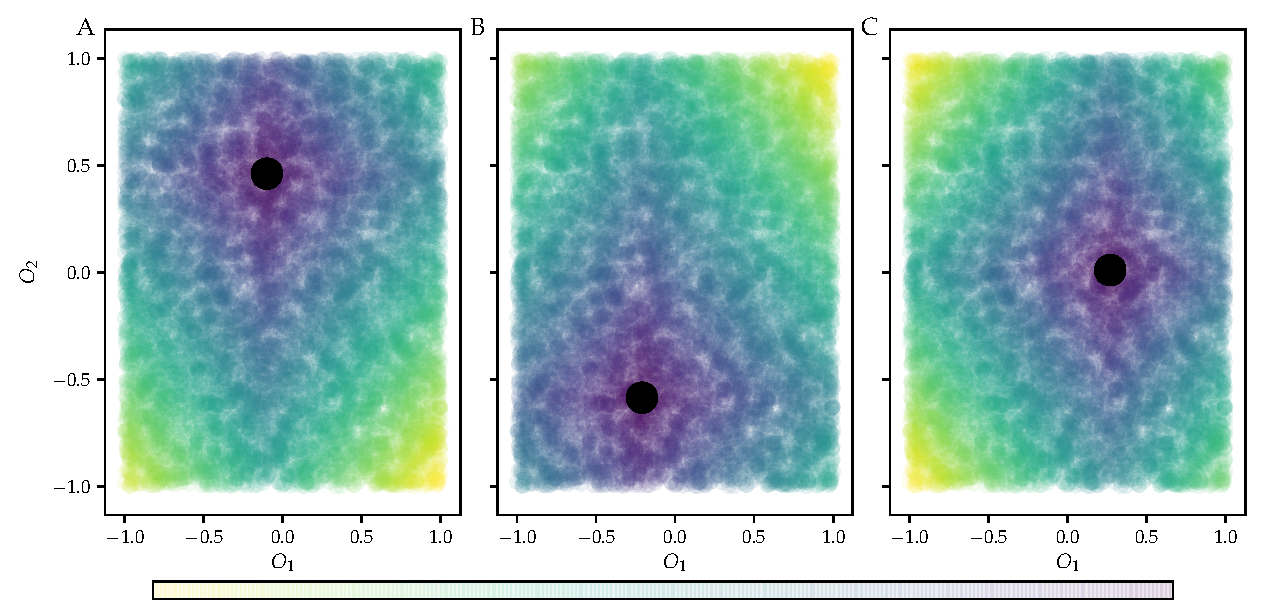
\includegraphics[width=1\textwidth]{../src/figs/rc-gen_anecdotal_comparison-2D.pdf}\vspace{-4mm}
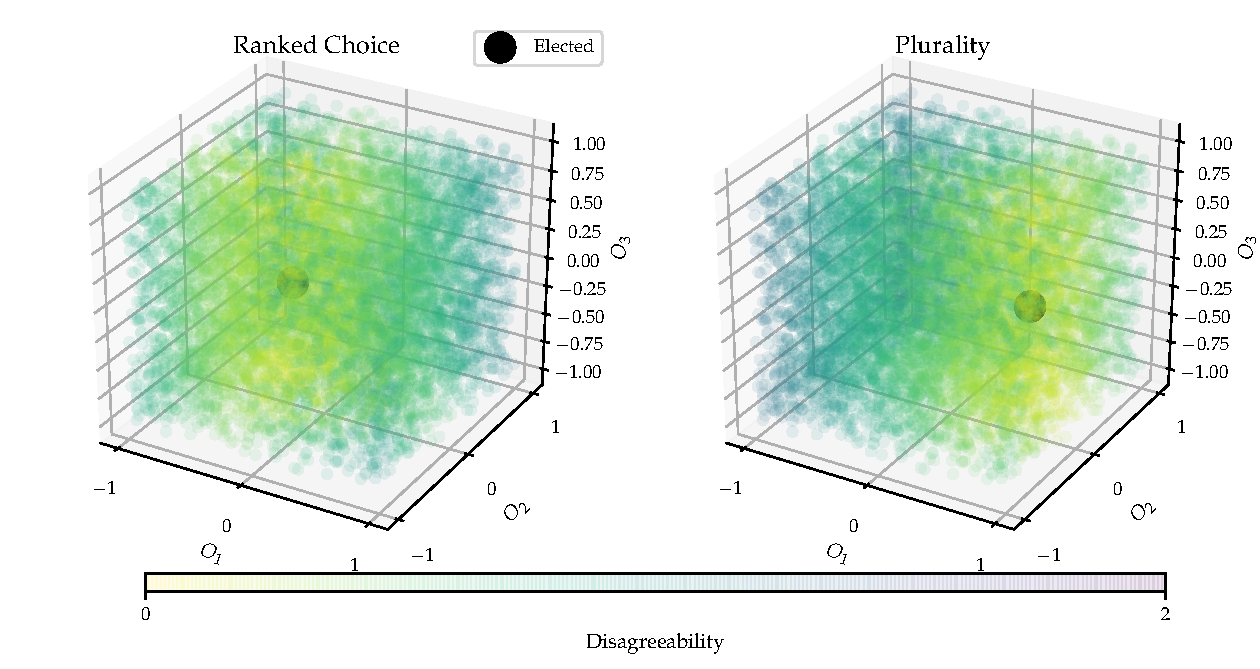
\includegraphics[width=1\textwidth]{../src/figs/rc-gen_anecdotal_comparison-3D.pdf}
\caption{Elected candidate in 2D and 3D opinion space for a single sample population, comparing ranked-choice outcome to plurality outcome.}
\label{fig:plurality_vs_rc_anecdotal}
\end{figure*}
